% Multiple Choice Question 20 to 21 (2 questions)

\textbf{See the instruction for questions \inteval{\value{question}+1} to \inteval{\value{question}+2}.}

\begin{center}
    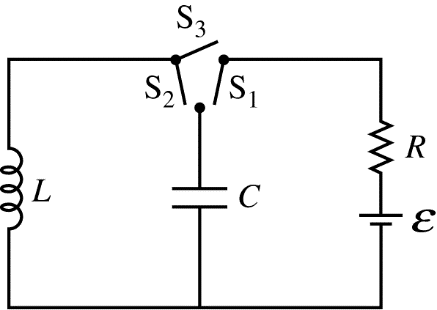
\includegraphics[scale=0.3]{images/img-011-019.png}
\end{center}

A circuit is constructed using a battery of emf $\mathcal{E}$, a resistor of resistance $R$, a capacitor of capacitance $C$, an inductor of inductance $L$, and three switches, as shown in the figure above. The three switches are labeled $\mathrm{S}_{1}, \mathrm{~S}_{2}$, and $\mathrm{S}_{3}$, and they can be operated independently.

% Multiple Choice Question 20
\begin{questions}\setcounter{question}{19}\question
All switches are open, and there is no stored energy in the capacitor or the inductor. Switch $S_{3}$ is closed. What is the current in the inductor after steady state has been reached?

\begin{oneparchoices}
    \choice $\dfrac{\mathcal{E}}{L R}$
    \choice $\dfrac{\mathcal{E}R}{L}$
    \choice $\dfrac{\mathcal{E}L}{R}$
    \choice $\dfrac{\mathcal{E}}{R}$
    \choice Zero
\end{oneparchoices}
\end{questions}

% Multiple Choice Question 21
\begin{questions}\setcounter{question}{20}\question
All switches are open, and there is no stored energy in the capacitor or the inductor. Switch $\mathrm{S}_{1}$ is closed. After the capacitor is fully charged, switch $\mathrm{S}_{1}$ is opened and switch $\mathrm{S}_{2}$ is closed. Which of the following expressions represents the maximum current in the $L C$ circuit?

\begin{oneparchoices}
    \choice $\dfrac{\mathcal{E}}{R}$
    \choice $\mathcal{E} \sqrt{\frac{C}{L}}$
    \choice $\mathcal{E} \sqrt{\frac{L}{C}}$
    \choice $\dfrac{\mathcal{E}C}{L}$
    \choice $\dfrac{\mathcal{E}L}{C}$
\end{oneparchoices}
\end{questions}
